% ================================================================
% Neural Demand Paper — CF Endogeneity Tables (auto-generated)
% N_RUNS = 5
% ================================================================

\begin{table}[htbp]
  \centering
  \caption{Control-Function RMSE — CES DGP (mean $\pm$ SE, 5 runs)}
  \label{tab:cf_endogeneity_ces}
  \begin{threeparttable}
  \begin{tabular}{lcccc}
    \toprule
    \textbf{Model} & $\rho=0.0$ & $\rho=0.3$ & $\rho=0.6$ & $\rho=0.9$ \\
    \midrule
    Neural Demand (static) & $0.00038 \pm 0.00002$ & $0.00035 \pm 0.00002$ & $0.00042 \pm 0.00002$ & $0.00043 \pm 0.00004$ \\
    Neural Demand (CF) & $0.00041 \pm 0.00003$ & $0.00037 \pm 0.00002$ & $0.00036 \pm 0.00004$ & $0.00044 \pm 0.00006$ \\
    Neural Demand (habit) & {---} & {---} & {---} & {---} \\
    Neural Demand (habit, CF) & $0.00051 \pm 0.00004$ & $0.00052 \pm 0.00002$ & $0.00053 \pm 0.00003$ & $0.00051 \pm 0.00004$ \\
    \bottomrule
  \end{tabular}
  \begin{tablenotes}\small
    \item RMSE evaluated against structural (IV-purged) demand at test prices.
    \item $\rho$ = endogeneity strength; $\rho=0$ is fully exogenous.
  \end{tablenotes}
  \end{threeparttable}
\end{table}

\begin{table}[htbp]
  \centering
  \caption{Control-Function RMSE — Habit DGP (mean $\pm$ SE, 5 runs)}
  \label{tab:cf_endogeneity_habit}
  \begin{threeparttable}
  \begin{tabular}{lcccc}
    \toprule
    \textbf{Model} & $\rho=0.0$ & $\rho=0.3$ & $\rho=0.6$ & $\rho=0.9$ \\
    \midrule
    Neural Demand (static) & $0.02214 \pm 0.00076$ & $0.02110 \pm 0.00058$ & $0.02260 \pm 0.00102$ & $0.02180 \pm 0.00094$ \\
    Neural Demand (CF) & $0.02221 \pm 0.00086$ & $0.02113 \pm 0.00064$ & $0.02243 \pm 0.00099$ & $0.02249 \pm 0.00103$ \\
    Neural Demand (habit) & {---} & {---} & {---} & {---} \\
    Neural Demand (habit, CF) & $0.01858 \pm 0.00078$ & $0.01502 \pm 0.00054$ & $0.01483 \pm 0.00048$ & $0.01838 \pm 0.00121$ \\
    \bottomrule
  \end{tabular}
  \begin{tablenotes}\small
    \item RMSE evaluated against structural (IV-purged) demand at test prices.
    \item $\rho$ = endogeneity strength; $\rho=0$ is fully exogenous.
  \end{tablenotes}
  \end{threeparttable}
\end{table}

\begin{figure}[htbp]
  \centering
  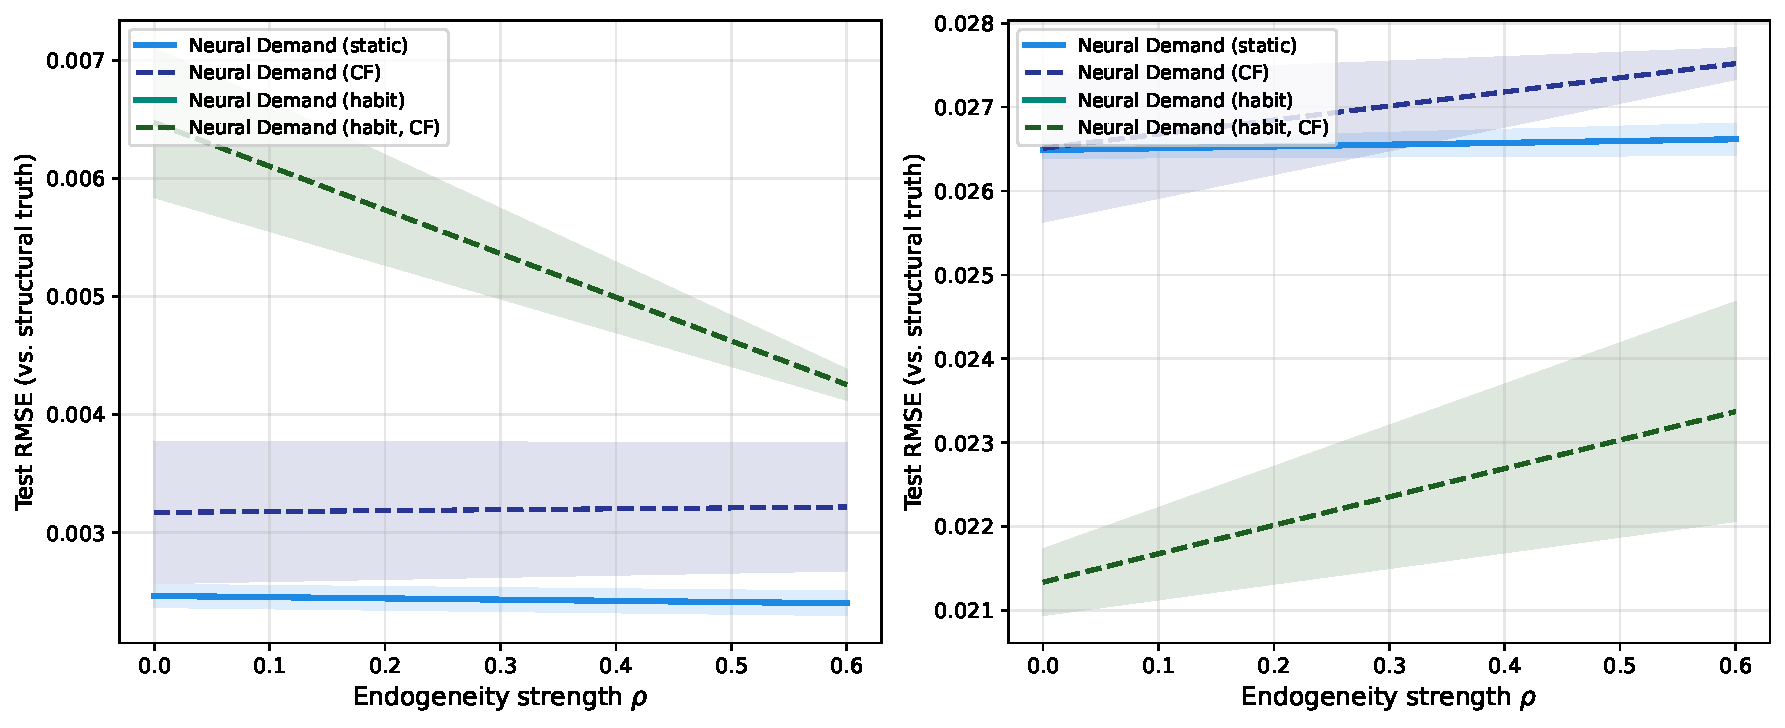
\includegraphics[width=0.85\linewidth]{results/neural_demand/simulations/figures/fig_cf_bias_reduction.pdf}
  \caption{RMSE vs.\ endogeneity strength $\rho$.  CF-corrected models (dashed) recover structural demand even at high $\rho$.}
  \label{fig:cf_bias_reduction}
\end{figure}

\begin{figure}[htbp]
  \centering
  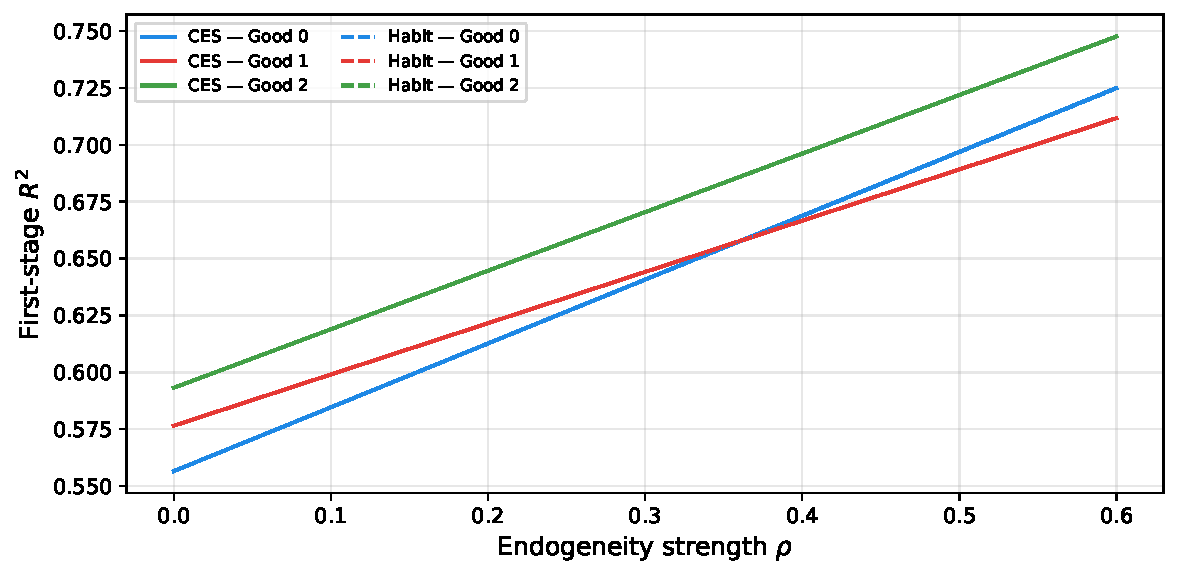
\includegraphics[width=0.85\linewidth]{results/neural_demand/simulations/figures/fig_cf_first_stage_rsq.pdf}
  \caption{First-stage $R^2$ for each good as a function of $\rho$, confirming instrument relevance.}
  \label{fig:cf_first_stage_rsq}
\end{figure}
